% The keyhole contour: an outer circle gamma joined by a thin corridor to a
% small inner circle (run clockwise) around the point a.
% Source: book/tex/complex-ana/holomorphic.tex (section: Cauchy's integral theorem).
\documentclass[border=2mm]{standalone}
\usepackage{tikz}
\usetikzlibrary{arrows.meta, decorations.markings, calc}
\begin{document}
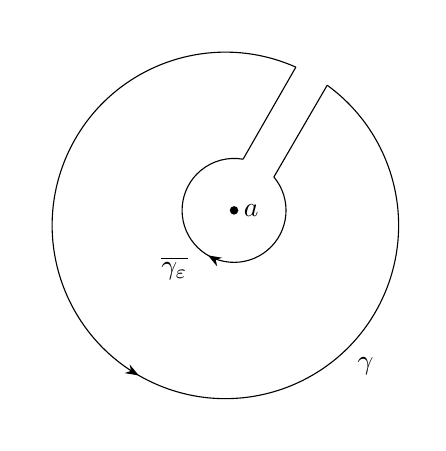
\begin{tikzpicture}[scale=2.2,
    decoration={markings, mark=at position 0.5 with {\arrow{Stealth}}}]
  \coordinate (a) at (60:0.1);
  \fill (a) circle (0.7pt) node[right] {$a$};
  % Outer circle, gap near 60 degrees.
  \draw[postaction={decorate}] (66:1) arc (66:414:1);
  % Inner circle around a (clockwise), gap near 60 degrees.
  \draw[postaction={decorate}] ($(a)+(40:0.3)$) arc (40:-280:0.3);
  % Corridor connecting the two gaps.
  \draw (54:1) -- ($(a)+(40:0.3)$);
  \draw ($(a)+(80:0.3)$) -- (66:1);
  \node at (-45:1) [below right] {$\gamma$};
  \node at ($(a)+(225:0.3)$) [below left] {$\overline{\gamma_\varepsilon}$};
\end{tikzpicture}
\end{document}
